
\documentclass[a4paper]{article}

\usepackage{url}

\usepackage[14pt]{extsizes}
\usepackage[
    left=20mm, top=15mm, right=15mm, bottom=15mm,
    nohead, footskip=10mm
]{geometry}
\usepackage[pdftex]{graphicx}

\usepackage[russian]{babel}
\usepackage[T2A]{fontenc}
% \usepackage{fontspec}
% \setmainfont{FreeSerif}
\usepackage{amssymb}
\usepackage{listings}
\usepackage{tabularx}
\newcolumntype{b}{X}
\newcolumntype{s}{>{\hsize=.5\hsize}X}

\usepackage{setspace,amsmath}




\begin{document}

\begin{center}
    \textbf{ПРАВИТЕЛЬСТВО РОССИЙСКОЙ ФЕДЕРАЦИИ} \\
    \textbf{НАЦИОНАЛЬНЫЙ ИССЛЕДОВАТЕЛЬСКИЙ УНИВЕРСИТЕТ} \\
    \textbf{«ВЫСШАЯ ШКОЛА ЭКОНОМИКИ»} \\
    \hfill\break
    \normalsize{Факультет компьютерных наук} \\
    Образовательная программа «Прикладная математика и информатика» \\
    \vspace{4.2cm}
    \textbf{Отчет об программном проекте} \\
    \hfill\break
    на тему Подготовка задач для олимпиады <<Высшая проба>> \\
\end{center}
\vspace{3cm}
\textbf{Выполнил:} \\
Студент группы БПМИ181 \hfill \underline{\hspace{5cm}} \hfill М. Деб Натх \\
\vspace{0.1cm} \\
\hspace*{\fill} Дата \;\underline{\hspace{4cm}}\; 2020 \\
\vspace{0.1cm} \\
\textbf{Принял:} \\
Руководитель проекта \hfill Густокашин Михаил Сергеевич
\begin{flushright}
    Директор \\
    Центра студенческих олимпиад ФКН НИУ ВШЭ
\end{flushright}
\vspace{0.5cm}
Дата \;\underline{\hspace{4cm}}\; 2020 \hfill
Оценка \quad \underline{\hspace{1.5cm}} \hfill
\underline{\hspace{5cm}} \\
\vfill
\begin{center}
    \textbf{Москва 2020}
\end{center}
\thispagestyle{empty}

\newpage

\section{Реферат}

Проведённая работа имела своей целью подготовку алгоритмических задач для проведения школьных олимпиад <<Высшая проба по информатике>> и <<Московская олимпиада школьников по информатике>> (обе проводились центром студенческих олимпиад НИУ ВШЭ). Результатом работы являются три подготовленные задачи, каждая из которых была предложена участникам олимпиад, а именно, отборочного и финального туров московской олимпиады школьников и отборочного тура олимпиады <<Высшая проба>>. 

Каждая из этих задач была протестирована членами методической комиссии данной олимпиады, после чего была предложена участникам. Написанный код успешно справился со своей задачей, так как во время проведения туров олимпиад, на которых были даны приготовленные в рамках данного проекта задачи, не возникло технических трудностей на стороне организаторов олимпиады, связанных с подготовленными задачами. Результаты работы написанных программ были использованы при оценивании решений участников олимпиады, ранжирования их и в конечном итоге -- награждения победителей дипломам ВСОШ.


\newpage

\tableofcontents


\newpage

\section{Введение}

\subsection{Краткое описание предметной области}

Предметная область проекта~--- разработка задач для соревнований по программированию, в том числе состязаний для школьников по программированию, проводимых НИУ ВШЭ, а именно, <<Высшая проба по информатике>>, <<Московская олимпиада школьников по информатике>> .

\subsection{Актуальность проблемы}

Создание качественных задач по программированию является актуальной задачей, так как с ростом популярности состязательного программирования растёт и нужда в разнообразных и оригинальных задачах, для решения которых могут потребоваться знания компьютерных наук, смежных им областей математики, знание языков программирования и умение написания программ.
Проведение олимпиад с задачами, удовлетворяющими вышеописанным требованиям является важной задачей, так как олимпиады <<Высшая проба>> и <<Московская олимпиада по информатике>> включены в Перечень олимпиад школьников, дающих льготы при поступлении в высшие учебные заведения РФ, в том числе и НИУ ВШЭ. Статус победителя этих олимпиад даёт право на поступление на ФКН без вступительных испытаний.

\subsection{Цель и задачи проекта}

Целью проекта была подготовка пакета нескольких задач по спортивному программированию, включающих в себя, но не ограничивающими следующими составными частями:
\begin{enumerate}
\item Условие задачи -- набранное в системе вёрстки \LaTeX условие, описывающее преамбулу задачи, формат входных и выходных данных, ограничения на входные данные.
\item Проверяющая программа (checker) -- программа, сверяющая вывод на конкретном тестовом примере ответ участника и ответ жюри, выводящая вердикт по данному тестовому примеру.
\item Главное авторское решение -- программа, оптимально решающая данную задачу, с выводом которой будет сверяться вывод участника.
\item Частичные решения -- либо правильные, но неоптимальные программы, либо неправильные программы, которые не проходят все тесты. Нужны для валидации корректности собранного пакета.
\item Валидатор (validator) -- программа, проверяющая корректность формата входных данных
\item Тесты -- набор тестовых входных данных и сгенерированный к ним набор выходных данных
\item Генераторы (generators) программы, генерирующие по входным аргументам тестовые примеры.
\end{enumerate}

\newpage
\section{Обзор и сравнительный анализ источников и аналогов}

\subsection{Аналоги}

Так как ежегодно проводятся сотни состязаний по спортивному программированию -- как онлайн-соревнования на платформах Codeforces \cite{Codeforces}, Timus \cite{Timus}, Codechief \cite{Codechief}, TopCoder\cite{TopCoder}, так и оффлайн-мероприятия, такие как Yandex.Algorithm \cite{YaAlgorithm}, Google Code Jam \cite{CodeJam}, Всероссийская олимпиада школьников по программированию \cite{Roi}, Facebook Hacker Cup.

В силу специфики проекта не представляется возможным переиспользование уже использованных задач -- это нарушит основополагающие правила проведения олимпиад и уничтожит соревновательный аспект состязания. 

\subsection{Выбранные методы для разработки проекта}


В силу технологических особенностей олимпиада <<Высшая проба>> проводится на платформе  ejudge, развёрнутой на сервере НИУ ВШЭ, а <<Московская олимпиада школьников>> проводится на платформе Yandex.Contest, развёрнутой на серверах Яндекса. Это ограничивает возможность использования иных форматов, кроме тех, что поддерживают эти системы. Поэтому было принято решение для хранения пакета использовать форматы систем Яндекс.Контест \cite{YaContest} и
Codeforces Polygon \cite{Polygon}.

Codeforces Polygon -- система подготовки задач, представленная командой разработки системы проведения соревнований codeforces.com \cite{Codeforces}. Является де-факто стандартом подготовки олимпиадных задач, импортирование пакетов задач формате роlуgоп поддерживается на основные решения для проведения олимпиад по программированию -- ejudge \cite{Ejudge}, codeforces \cite{Codeforces}, Yandex Contest \cite{YaContest}. Именно широкая поддержка этого формата разными платформами и послужила причиной выбора этой системы для разработки пакетов задач. 

\subsection{Функциональные и нефункциональные требования к программному проекту}

В связи с вышеописанными технологическими ограничениями складывается единственное функциональное требование -- работоспособность при использовании системой подготовленного пакета задач, выражающаяся в возможности отправить произвольное решение в систему по подготовленной задаче и получит один из следующих вердиктов:
\begin{enumerate}
\item    \texttt{OK}~--- OK, Решение является полным
\item    \texttt{CE}~--- Compilation Error, Ошибка компиляции
\item    \texttt{RT}~--- Run-Time Error, Ошибка при работе программы
\item    \texttt{TL}~--- Time-Limit Exceeded, Ошибка превышения лимита времени
\item    \texttt{PE}~--- Presentation Error, Ошибка неправильного формата результата
\item    \texttt{WA}~--- Wrong Answer, Неправильный ответ
\end{enumerate}
Описанные выше вердикты продиктованы функциональными особенностями систем и общепринятыми стандартами.

В качестве нефункциональных требований к подготавливаемым задачам можно выделить то, чтобы задача в своём решении требовала от участника знаний в использовании алгоритмов и структур данных, умения пользоваться языками программирования, а решение задачи было нетривиально и требовало как творческого, так и математического мышления.

\newpage

\section{Теоретическая часть. Описание выбранных методов, алгоритмов и методик}

\subsection{Задача №1}

Первой задачей, подготовленной в рамках данного проекта была задача <<C>> (нумерация задач в мире спортивного программирования традиционно буквенная) со второго отборочного этапа олимпиады <<Высшая проба>>. Этот этап проходил в качестве онлайн-тура длительностью 3 часа на платформе ejudge. Ниже приведены условия и решения задачи, важные аспекты реализации приведены в секции \ref{realise.1}

\subsubsection{Условие задачи}

В условии этой задачи дана полоска (матрица) натуральных чисел размера $N \times 2$ и натуральное число $K$.

Требуется разместить на данной полоске ровно $K$ непересекающихся доминошек (матриц $2\times1$ или $1\times 2$) таким образом, чтобы сумма чисел на не покрытых доминошками клеток была минимально. Доминошки можно поворачивать горизонтально или вертикально, они не могут накладываться. Обязательно использовать все имеющиеся доминошки.

Требуется определить, как именно надо расположить доминошки для минимизации целевой функции и вывести любую найденную конфигурацию, на которой достигается этот минимум.

\textbf{Ограничения на входные данные:}
\begin{itemize}
    \item $1 \leqslant N \leqslant 2 \cdot 10^{5}$;
    \item $0 \leqslant K \leqslant 2 \cdot 10^{5}$;
    \item $0 \leqslant N \times K \leqslant 2 \cdot 10^{5}$;
    \item $N \geqslant K$;
\end{itemize}

\textbf{Ограничения на решение задачи:}
\begin{itemize}
    \item Ограничение по виртуальной памяти, которую использует решение участника: 256MB
    \item Ограничение по виртуальному времени, которое использует решение участника: 1 сек.
\end{itemize}

Оценка потестовая, а именно, в задаче ровно $30$ тестов, за прохождение каждого из них участнику начисляется один балл. Решение, правильно работающее при ограничениях $N \leq 20$ будет набирать не менее 15 баллов.

% Ниже приведён пример входных и выходных данных к этой задаче:

% \begin{table}[htbp]
%     \centering
%     \begin{tabularx}{\textwidth}{|c|c|}
%     % \begin{tabularx}{\textwidth}{bss}
%         \hline
%         \texttt{стандартный ввод} & \texttt{стандартный вывод}       \\ \hline
%         0         & 2              \\ \hline
%         1         & 3              \\ \hline
%     \end{tabularx}
% \end{table}




\subsubsection{Решение задачи}

Для решения этой задачи участнику предлагалось либо реализовать полный перебор (для получения 15 баллов), либо воспользоваться методом динамического программирования для полного решения.

В первую очередь заметим, что задача минимизации суммы непокрытых клеток равносильна задаче максимизации суммы покрытых клеток, так как их общая сумма есть константа -- сумма всех чисел в таблице.

По своей сути динамическое программирование -- это метод математической индукции или рекурсивная формула, реализованная программно. 
Динамическое программирование в спортивном программировании -- способ решения сложных задач путём разбиения их на более простые подзадачи. Динамическое программирование представляет из себя переформулирование сложной задачи в виде рекурсивной последовательности более простых подзадач. Простейшим примером применения динамического программирования можно считать алгоритм линейного вычисления $n$-го числа Фибоначчи.

В данном случае предлагалось использовать то, что называется многомерным динамическим программированием~--- подвидом д.п., при котором подзадача описывается более чем одним параметром.

Обозначим за \texttt{dp[k][i][j]}, где $0 \leq i \leq N$, $0 \leq j \leq K$, $0 \leq k \leq 3$ число, равное максимальной сумме покрытых клеток, если рассматривается задача покрытия первых $i$ столбцов $j$ доминошками, при этом в последнем столбце:
\begin{itemize} 
    \item ни одна клетка не покрыта, если $k = 0$;
    \item только верхняя клетка покрыта, если $k = 1$;
    \item только нижняя клетка покрыта, если $k = 2$;
    \item обе клетки покрыты, если $k = 3$;
\end{itemize} 

Тогда нетрудно видеть рекурсивную формулу для этих величин: Если обозначить данный двумерный массив за \texttt{A}, то 

\begin{lstlisting}
dp[0][i][j] = max(
    dp[0][i-1][j],
    dp[1][i-1][j],
    dp[2][i-1][j],
    dp[3][i-1][j]
);

dp[1][i][j] = max(
    dp[0][i-1][j-1],
    dp[2][i-1][j-1]
) + A[i][0] + A[i-1][0];

dp[2][i][j] = max(
    dp[0][i-1][j-1],
    dp[1][i-1][j-1]
) + A[i][1] + A[i-1][1];

dp[3][i][j] = max(
    dp[0][i-1][j-1],
    dp[1][i-1][j-1],
    dp[2][i-1][j-1],
    dp[3][i-1][j-1]
) + A[i][0] + A[i][1];
\end{lstlisting}

С помощью такой рекурсивной формулы, положив изначально \texttt{dp[k][i][j]}$=+\infty$, а также     \texttt{dp[0][0][0] = 0;}\texttt{dp[3][0][1] = A[0][0] + A[0][1];}, можем за $\mathcal O(NK)$ вычислить все значения \texttt{dp} и ответ в таком случае будет равен $\max\limits_{0 \leq k \leq 3}$\texttt{dp[k][N][K]}. На языках C, C++, Java, Pascal такое решение будет укладываться в указанные ограничения по памяти и времени.




\newpage
\subsection{Задача №2}
Задачи 2 и 3 являли собой задачи с открытыми тестами -- такой формат часто используется на Московской олимпиаде по программированию. Это значит, что тесты известны участнику и его задача -- лишь найти ответы к данным тестам. Часто задачи с открытыми тестами бывают оптимизационными задачами -- когда точный ответ неизвестен и работа участника оценивается в сравнении с решениями жюри и других участников -- чем ближе к максимальному известному ответу участник смог найти решение, тем выше его балл

Вторая задача была предложена на втором отборочном этапе олимпиады <<Московская олимпиада школьников>> для учащихся 10-11 классов. Раунд проходил на платформе Яндекс.Контест и длился несколько дней.

\subsubsection{Условие задачи}

Вторая задача была реализацией известной NP-полной задачи SETCOV, ниже приведена её формулировка:

Дано множество $A$ из $n$ элементов (все элементы -- числа от 1 до $n$). Также есть семейство $B$ из  $m$ подмножеств. $i$-е подмножество содержит ровно $k_i$ элементов, равных $x_{i\, 1}, x_{i\, 2}, \ldots x_{i\, k_i}$. Разумеется, один элемент может быть выбран не более чем в одно множество. Задача ~--- выбрать какой-то поднабор подмножеств из данного семейства $B$ таким образом, чтобы каждый элемент из $A$ присутствовал не более чем в одном множестве из $B$, при этом максимизировав число выбранных элементов $t$.


\subsubsection{Решение задачи}

Не было зафиксировано какое-то конкретное решение, так как задача носила оптимизационный характер -- участник, нашедший решение, максимизирующее $t$ и получал максимальный балл. Поэтому в решении данной задачи были использованы классические методы оптимизации~--- метод локальной оптимизации, метод имитации отжига, а в некоторых случая -- полный перебор.

Участнику предлагалось самому проанализировать входной набор тестов и заметить, что тесты, которые можно было гарантированно решить с помощью тривиального полного перебора за $\mathcal O(n2^m)$ составляли 30\% тестов задачи, остальные тесты с достаточно большими ограничениями -- остальные 70\%

\newpage
\subsection{Задача №3}

Третья задача, как и вторая носила оптимизационный характер и имела открытые тесты, хотя авторское решение этой задачи предполагало нахождение полного ответа, гарантированного корректного и оптимального.

Задача была предложена участникам заключительного этапа <<Московской олимпиады школьников>> для учащихся 10-11 классов. Раунд проходил на платформе Яндекс.Контест и длился 4 часа. Изначально запланированный как оффлайн-турнир с точкой проведения в Москве, его в связи с ограничительными эпидемиологическими мерами пришлось провести онлайн с системой прокторинга. 


\subsubsection{Условие задачи}

Sokoban (Soko-Ban, яп.~--- «кладовщик»)~--- логическая игра-головоломка, в которой игрок передвигает ящики по лабиринту, показанному в виде плана, с целью поставить все ящики на заданные конечные позиции. 


Для этого пользователь перемещает человека, которого мы называем Сокобан. Сокобан может двигаться вверх, вниз, влево и вправо. Он не может проходить сквозь стены или ящики. Он может толкать только одну коробку за раз (никогда не тянуть). В любое время квадрат может быть занят только одной стеной, коробкой или Сокобаном.

Более формально, вам изначально известная конфигурация лабиринта~--- поля $n\times m$, состоящая из пустых клеток или стен. Также вам известна начальная позиция каждого из ящиков, конечные позиции, куда надо поставить ящики и начальное положение Сокобана.

Участнику предлагалось найти кратчайший способ решить головоломку -- найти наиболее короткий способ поставить все ящики на позиции.





\subsubsection{Решение задачи}

Предполагалось, что эта задача требует умение пользоваться базовыми алгоритмами на графах и умение быстро писать код. Авторское решение использует алгоритм BFS (поиск в глубину)~--- рассматривается граф, состоящий из всевозможных конфигураций (конфигурация -- это совокупность положений ящика и сокобана), где ребро ставится из вершины $A$ в вершину $B$ тогда и только тогда, когда из конфигурации $A$ при шаге сокобана в одном из направлений, лабиринт перейдёт в состояние B. 

Затем можно было воспользоваться общими идеями о данной игре -- например, если ящик стоит в углу, то он останется там стоять и данная конфигурация не приведёт к решению и её можно выбросить.

Такое решение, аккуратно написанное набирало 30\% баллов.

Решением на 70\% была оптимизация написанного выше с использованием оптимизации BFS, известной также как метод meet-in-the-middle~--- вместо запуска из стартовой конфигурации алгоритм запускается одновременно из стартовой и конечной конфигурации и два поиска работают параллельно, затем, если они обе найдут кратчайший путь до какой-то вершины $v$, то будет найден кратчайший путь до вершины $v$ из стартовой вершины и кратчайший путь до конечной вершины из вершины $v$, а значит, будет найден кратчайший путь из стартовой в конечную вершину.

Авторское решение работало около 8 минут и потребляло $1.5$Гб оперативной памяти~--- предполагалось, что участники напишут решения, время работы которых займёт не более $30$ минут и не более $3$Гб оперативной памяти.

Ниже приведён пример решения головоломки Сокобан для лучшего понимания формулировки задачи

\begin{figure}[ht]
\begin{center}
   \makebox[\linewidth][c]{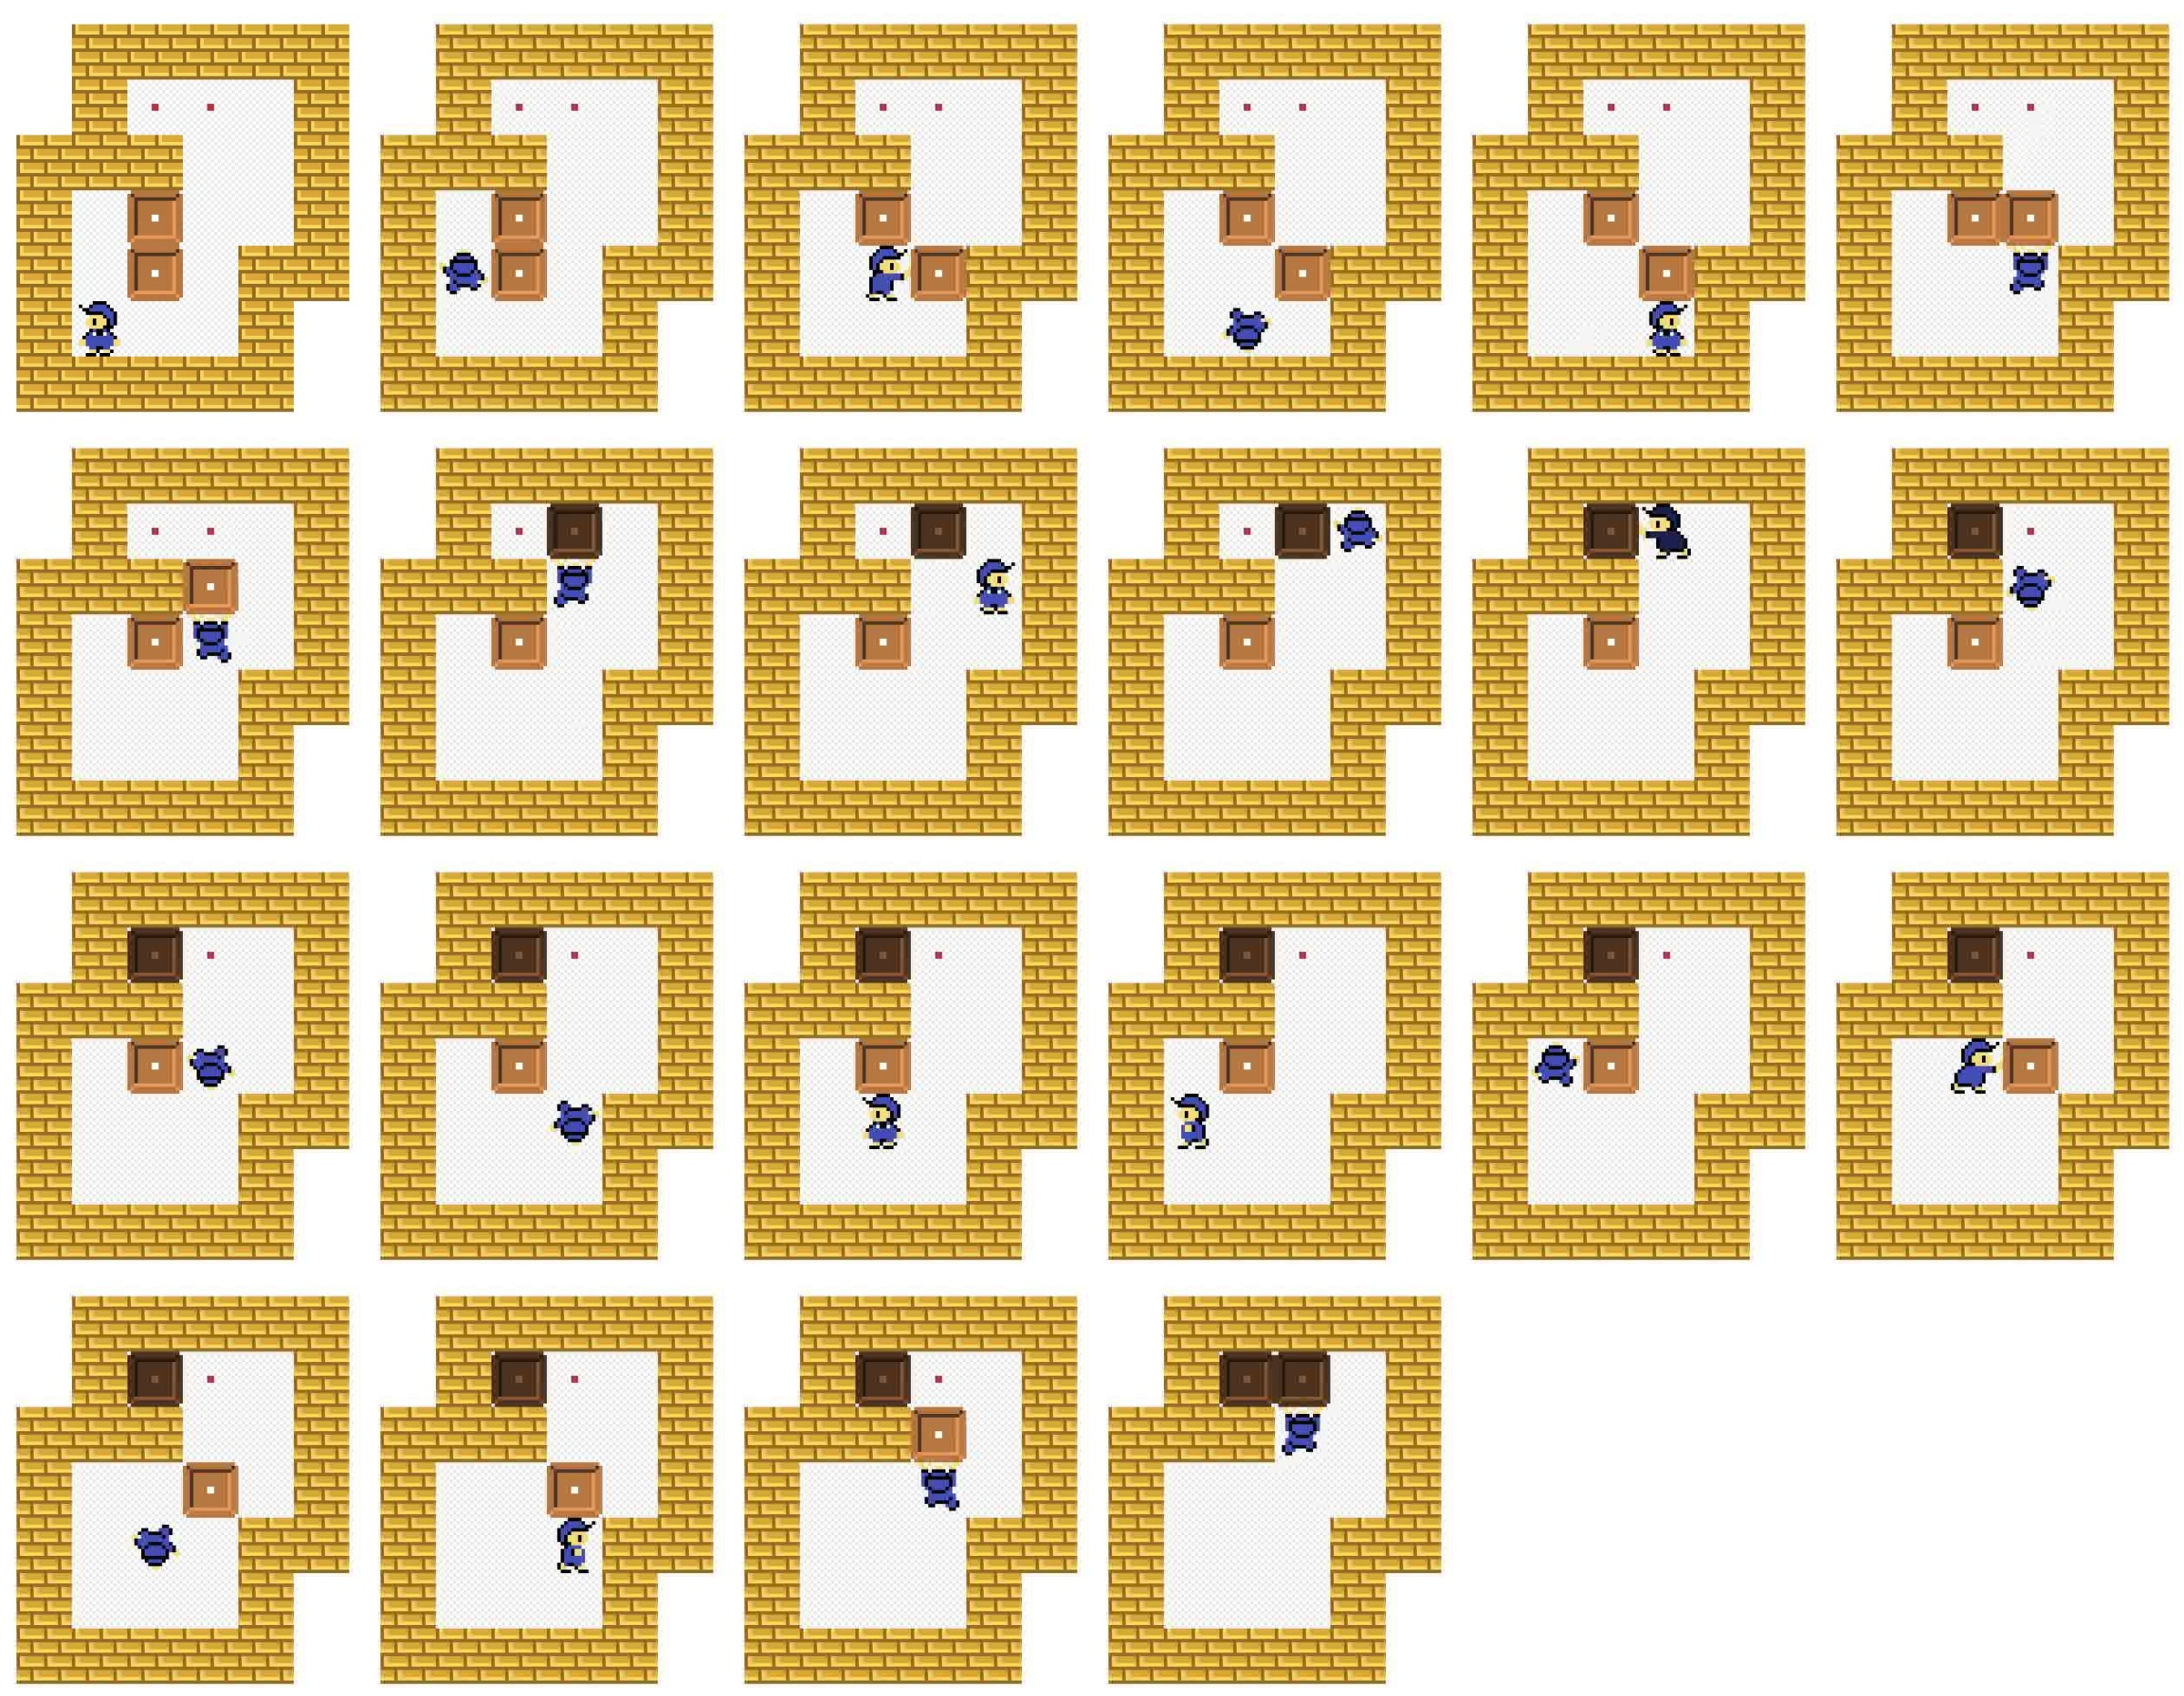
\includegraphics[width=0.8\textwidth]{../mosinf-sokoban/statement/example-sokoban.jpg}}
\end{center}
\end{figure}

 
\newpage
\section{Реализация проекта}

Все исходные файлы можно найти в github-репозитории \url{https://github.com/DebNatkh/hse-project/}.

\subsection{Задача №1}\label{realise.1}

В данной задаче было написано решение, работающее за $\mathcal O(nk)$, описанное выше, а также были написана тривиальные валидаторы и чекеры -- сравнивающие найденные ответы и проверяющие найденные ответы на валидность. Также был написан генератор случайных тестов \texttt{gen}.

Он принимает 4 аргумента $N$, $K$, $type$, $M$, где $N$, $K$ соответствуют условию, а $type$ указывает, будут ли все элементы матрицы равны между собой, где $M$~--- максимально допустимое число в матрице. Генератор был запущен 30 раз для генерации 30 различных тестов:

\texttt{gen 5 0 random }

\texttt{gen 5 3 random }

\texttt{gen 15 10 random }

\texttt{gen 20 5 random 300 }

\texttt{gen 20 1 random }

\texttt{gen 20 3 random }

\texttt{gen 20 10 random }

\texttt{gen 20 13 random }

\texttt{gen 20 15 random }

\texttt{gen 20 15 random 1 }

\texttt{gen 20 17 random 1 }

\texttt{gen 20 19 random 300 }

\texttt{gen 20 20 random }

\texttt{gen 20 20 random 300 }

\texttt{gen 20 20 equal }

\texttt{gen 10000 5 random }

\texttt{gen 1000 30 random }

\texttt{gen 1000 200 random }

\texttt{gen 1000 200 random 5 }

\texttt{gen 1000 200 equal }

\texttt{gen 2000 50 random }

\texttt{gen 2000 75 random }

\texttt{gen 2000 100 random }

\texttt{gen 5000 20 random }

\texttt{gen 5000 40 random }

\texttt{gen 100000 2 random }

\texttt{gen 50000 4 random }

\texttt{gen 50000 4 random 4 }

\texttt{gen 50000 4 equal }

\texttt{gen 100000 1 random }


\newpage

\subsection{Задача №2}

Как сказано выше, было написано несколько решений от полного перебора до алгоритма имитации отжига, каждый из которых максимизировал целевой функционал. Для генерации тестов была использована написанная утилита \texttt{gen}, принимающая три параметра $n$, $m$, $k$, где $n$--- число элементов, $m$~--- число множеств, а размер каждого из множеств выбирался из случайного распределения $\mathcal{N} (k, \operatorname{rand})$, где $rand$~--- случайное целое число от $1$ до $10$.

Было сделано 6 тестов, решающихся с помощью полного перебора:

\texttt{gen 5 5 3}

\texttt{gen 10 10 5}

\texttt{gen 20 15 5}

\texttt{gen 100 20 5}

\texttt{gen 100 20 10}

\texttt{gen 100 20 15}


и 14 тестов, где необходимо было использовать методы оптимизации:

\texttt{gen 20 20 4}

\texttt{gen 20 40 6}

\texttt{gen 20 60 8}

\texttt{gen 20 100 10}

\texttt{gen 20 100 10}

\texttt{gen 24 100 10}

\texttt{gen 10000 10 12}

\texttt{gen 10000 11 40}

\texttt{gen 1000 30 10}

\texttt{gen 1000 60 10}

\texttt{gen 1000 60 2}

\texttt{gen 9999 100 78}

\texttt{gen 10000 100 30}


Формула $5 \times\left(\frac{\text {ParticipantSolution}}{\text {BestSolution}}\right)^{3}$ была выбрана в качестве формулы оценки за каждый из тестов, где $\text{ParticipantSolution}$~--- суммарное число занятых аудиторий в решении участника, а $\text{BestSolution}$~--- суммарное число занятых аудиторий в лучшем среди участников и жюри решении. При тестировании этой формулы и различных частичных решений использование именно такой формулы показалось целесообразным и справедливым в оценивании.

\newpage

\subsection{Задача №3}

Для проверки задачи был написан код, который эмулировал логику игры sokoban и на каждое решение участника выдавал вердикт, верно ли был решён каждый из тестов.


Для решения задачи был написан код, реализующий BFS с meet-in-the-middle, затем для генерации тестов были выбраны уже известные головоломки сокобан, собранные в разные архивы, таких тестов было порядка 3 тысяч. Затем авторское решение было протестировано на каждом из них, замеряя время работы обычного BFS, двухстороннего BFS, а также объём потребляемой памяти. После этого в первую группу тестов (15 штук) были отобраны тесты, суммарное время работы на которых обычного BFS не превосходило 2 минут. Во вторую группу тестов (25 штук) были отобраны тесты, суммарное время работы полного решения  на которых не превосходило 8 минут, и при этом решение с использование обычного BFS не работало в связи с ограничениями по памяти или времени.


Формула  $2 \times\left(\frac{\text {BestSolution}}{\text {ParticipantSolution}}\right)^{4}$была выбрана в качестве формулы оценки за каждый из тестов, где $\text{ParticipantSolution}$~--- длина кратчайшего решения, найденного участником, а $\text{BestSolution}$~--- длина кратчайшего решения, найденного  среди всех решений  участников и жюри. При тестировании этой формулы и различных частичных решений использование именно такой формулы показалось целесообразным и справедливым в оценивании.


\newpage
\section{Заключение}

Могу считать проект выполненным успешно -- все задачи были предложены нескольким сотням участников. Например, последнюю задачу пытались, хоть и безуспешно, решить 45 участников, в решении второй задаче было предпринято свыше 1900 посылок. Все олимпиады состоялись без каких-либо значимых форс-мажоров, что считаю критерием удачно проделанной работы.

Ниже привожу фрагмент турнирной таблицы отборочного этапа <<Московской олимпиады школьников>>, в которой задача D~--- это вторая приготовленная задача.

\begin{figure}[ht]
\begin{center}
   \makebox[\linewidth][c]{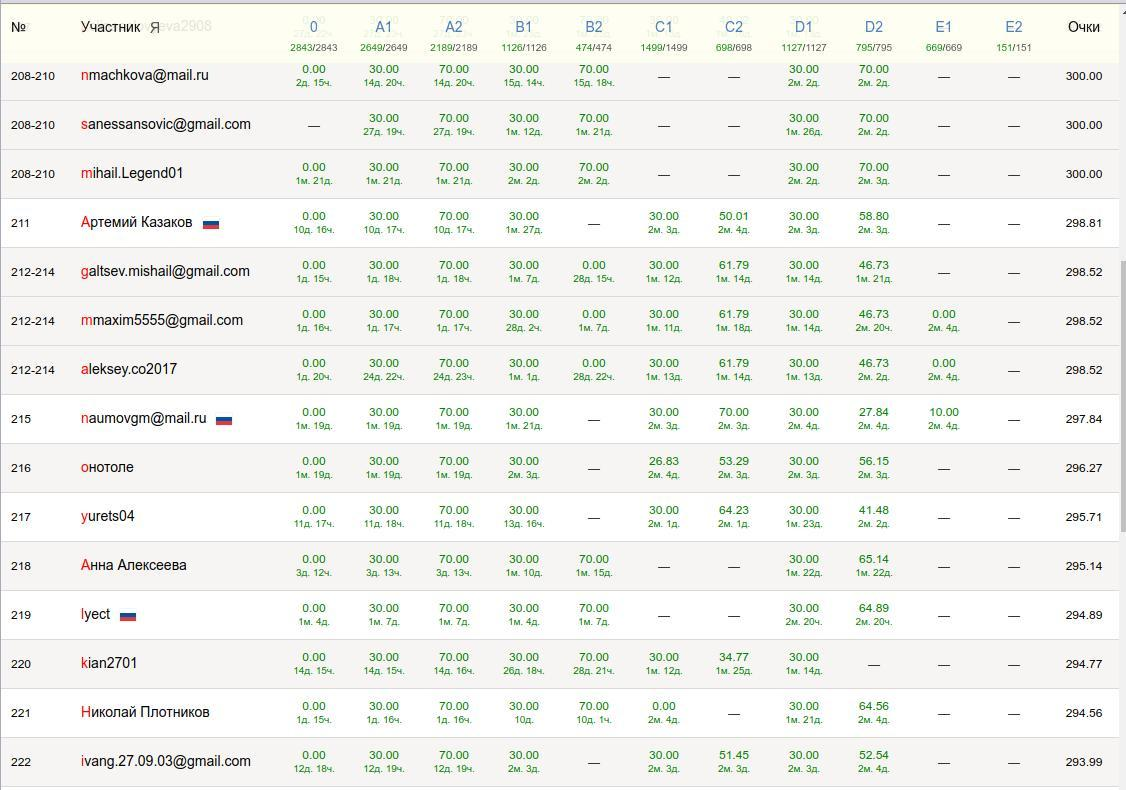
\includegraphics[width=\textwidth]{photo_2020-06-24_20-31-42.jpg}}
\end{center}
\end{figure}

\newpage


\begin{thebibliography}{3}
\bibitem{YaContest} Яндекс.Контест / Yandex.Contest, 
    \url{https://contest.yandex.ru/about/}
\bibitem{Polygon} Codeforces Polygon beta, 
    \url{https://polygon.codeforces.com/}
\bibitem{Codeforces} Codeforces, 
    \url{https://codeforces.com}
\bibitem{CodeChief} CodeChief, 
    \url{https://codechief.com}
\bibitem{Ejudge} Ejudge, 
    \url{https://ejudge.ru/}
\bibitem{HPArchive} Архивы прошлых лет всероссийской олимпиады школьников <<Высшая проба>> 
    \url{https://olymp.hse.ru/mmo/materials-it}
\bibitem{Timus} Timus ( Online Judge 
    \url{https://acm.timus.ru/?locale=ru}
\bibitem{Informatics} Сайт дистанционной подготовки к олимпиадам по программированию 
    \url{https://informatics.mccme.ru/}
\bibitem{YaAlgorithm} Yandex.Algorithm
    \url{https://contest.yandex.com/algorithm2017/}
\bibitem{TopCoder} TopCoder
    \url{https://www.topcoder.com/community/competitive-programming/}
\bibitem{Roi} Официальная страница Всероссийской олимпиады школьников по информатике (РОИ)
    \url{http://rosoi.net/2020/}
\bibitem{CodeJam} Google Code Jam
    \url{https://codingcompetitions.withgoogle.com/codejam}
\bibitem{MosInf} Московская олимпиада школьников по информатике
    \url{http://mos-inf.olimpiada.ru/}
\end{thebibliography}
\end{document}




\end{document}


% •      Титульный лист
% •      Реферат (0,5 - 1,0 страницы). Необходимо кратко описать объект исследования, цель работы, метод или методологию проведения работы, результаты работы, апробацию работы (публикации, выступления на конференциях, тезисы докладов, Свидетельства о регистрации программ и т.п.); перечень ключевых слов;
% •       Содержание с указанием номеров страниц;
% •       Введение (1,5 - 3 страницы). Краткое описание предметной области, актуальность проблемы, цель и задачи проекта;
% •       Обзор и сравнительный анализ источников и аналогов. На основе анализа источников выбрать методы / алгоритмы / модели для решения поставленных задач. На основе анализа аналогов сформулировать функциональные и нефункциональные требования к программному проекту.
% •      Теоретическая часть. Подробное описание выбранных и/или разработанных методов, алгоритмов, моделей данных, методик, и т.п.
% •      Реализация проекта:

%     Архитектура / структура проекта / программы,
%     Выбор средств, инструментов и технологий разработки,
%     Схема базы данных с описанием,
%     Описание серверной части проекта,
%     Описание клиентской части проекта,
%     Реализация основных алгоритмов,
%     Диаграмма классов, описание классов, ссылка на репозиторий с исходными кодами программы / классов,
%     Описание запуска программы (где ее скачать, где и как развернуть, как запустить, как выполнить основные функции)
%     Описание тестирования программы,
%     Анализ и оценка полученных результатов;
% •       Заключение: основные результаты и перспективы дальнейшей работы;
% •       Список использованных источников;
% •       Приложения (при необходимости). В приложения могут быть вынесены исходные коды полностью или частично, результаты испытаний, результаты экспериментов и т.п.



